\title{Problem Set I}
\author{
        Ethan Rooney \\
        Department of Physics\\
}
\date{\today}

\documentclass[12pt]{article}
\usepackage{amssymb}
\usepackage{amsmath}
\usepackage{cancel}
\usepackage{graphicx}
\usepackage[margin=1in]{geometry}
\begin{document}
\maketitle

\section{Proton Number, Neutron Number, Mass Number}
\begin{table}[h]
  \begin{tabular}{|l|l|l|l|l|}
    \hline
    {\bf Nuclei}        & {\bf Z}       & {\bf N }     & {\bf A }      & {\bf Applications} \\ \hline
    Carbon-14     & 6       & 8       & 14      & Radio-dating up to 50,000 years \\ \hline
    Phosphorus-32 & 15      & 17      & 32      & \begin{tabular}[t]{@{}l@{}}Radio-tagging DNA segments\\ 
                                                metabolic Pathway Tracing\end{tabular}\\ \hline
    Cobalt-60     & 27      & 33      & 60      & \begin{tabular}[t]{@{}l@{}}Hard Gamma Emitter \\
                                                Sterilize Medical Equipment \\
                                                My favorite isotope\end{tabular} \\ \hline
    Technetium-99 & 43      & 56      & 99      & \begin{tabular}[t]{@{}l@{}}Meta-Stable ($^{99m}$Tc) \\
                                                used widely for medical imaging\end{tabular} \\ \hline
    Lead-208      & 82      & 126     & 208     & \begin{tabular}[t]{@{}l@{}}Ratio of Pb-208:Pb-204 \\
                                                used to determine past presence \\
                                                Radio-Nuclides: Uranium/Thorium/Plutonium.\end{tabular} \\ \hline
    Radium-226    & 88      & 138     & 226     & \begin{tabular}[t]{@{}l@{}}Daughter of $^{238}$U Decay \\
                                                A Leading Cause of Lung Cancer \end{tabular} \\ \hline
    Uranium-235   & 92      & 143     & 235     & \begin{tabular}[t]{@{}l@{}}Naturally in Uranium Ore $0.72\%$ \\ 
                                                When Enriched to a high percent of Uranium \\
                                                Can be used on Nuclear Power Plants \\
                                                Or Nuclear Weapon\end{tabular} \\ \hline
  \end{tabular}
\end{table}
 
\begin{table}[h]
  \begin{tabular}{|c|l|l|l|}
    \hline
    \bf Reaction                                            & \bf Z                     & \bf N                       & \bf Pos \\\hline
    $^{226}Ra \rightarrow {}^{222}Rn + \alpha$              & $ 88 = 86 + 2 $           & $138 = 136 + 2$              & Yes \\\hline
    $^{235}U + n \rightarrow { }^{138}Xe + { }^{94}Sr + 4n$ & $ 92 + 1 \neq 54 + 38 + 0$& $143 + 0 \neq 84 + 56 + 4$  & No \\\hline
    $^{239}Pu \rightarrow {}^{140}Cs + {}^{98}Zr + n$       & $ 94 \neq 55 + 40 + 1 $   & $145 \neq 85+58+1 $         & No \\\hline
  \end{tabular}
\end{table}

\pagebreak
\section{Cyclotron}

Given: $p = 200 \textrm{MeV}$, $m = 938 \textrm{MeV}$, $\Delta{T}=100\textrm{KV}$, $k=e$
\begin{equation}
E^2 = p^2 + m^2
\end{equation}
\begin{equation}
T = E - m
\end{equation}
\begin{equation}
T = \sqrt{p^2+m^2}  - m
\end{equation}
\begin{equation}
  T = \sqrt{(200 \textrm{MeV})^2+(938 \textrm{MeV})^2}  - 938 \textrm{MeV} = 21.1\textrm{MeV} 
\end{equation}
\begin{equation}
  T = kn\Delta{T}
\end{equation}
\begin{equation}
  n = \frac{T}{k\Delta{T}} \frac{21.1 \textrm{MeV}}{e*100\textrm{KV}}= 211
\end{equation}
\begin{table}[h]
  \centering
  \begin{tabular}{|c|}
    \hline
      \bf 211 Revolutions \\
    \hline
  \end{tabular}
\end{table}

\pagebreak
\section{Cross section of a Disk}

\begin{figure}[h]
  \centering
  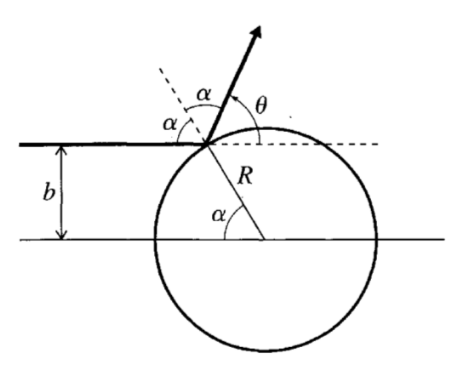
\includegraphics[width=200pt]{disk_scatter.png}
  \caption{Credit to http://web.physics.ucsb.edu/~fratus/phys103/LN/Scattering.pdf for image.}
  \label{fig:disk}
\end{figure}

A particle traveling towards a disk of radius $R$. Travelling parallel to an axis passing through the center of the disk. At a distance $b$ from the axis.

\begin{equation}
b=R{\sin{\alpha}}
\end{equation}
\begin{equation}
  \Theta=\pi-2\alpha
\end{equation}
\begin{equation}
  \alpha=\frac{\pi-\Theta}{2}
\end{equation}
\begin{equation}\label{eq:geometry}
  b=R\sin{\frac{\pi-\Theta}{2}}
\end{equation}
\begin{equation}
  \frac{{d}{b}}{{d}{\Theta}}=-\frac{R}{2}\sin{\frac{\Theta}{2}}
\end{equation}
\begin{equation}
  \int_{-2\pi}^{0}-\frac{R}{2}\sin{\frac{\Theta}{2}}=2R
\end{equation}
This means that for the entire scattering range, $b$ must cover the whole range of $(-R,R)$. Or that the target size is equal to the Length $2R$.

\pagebreak
\section{Spherical Cross Section}
We can plug equation \eqref{eq:geometry} into ${d}\sigma=b\cdot{d}b\cdot{d}\alpha$ to get:

\begin{equation}
  {d}\sigma=R\sin{\frac{\pi-\Theta}{2}}\cdot{d}b\cdot{d}\phi
\end{equation}

\begin{equation}
  \oint{d}\sigma=\int_0^{2\pi}\int_0^R R\sin{\frac{\pi-\Theta}{2}}\cdot{d}b\cdot{d}\phi
\end{equation}

\begin{equation}
  \sigma=2\pi R^2\sin{\frac{\pi-\Theta}{2}}
\end{equation}

\begin{equation}
  \frac{d\sigma}{d\Theta}=-\pi{R^2}\sin{\frac{\Theta}{2}}
\end{equation}

\begin{equation}
  \oint\frac{d\sigma}{d\Theta}=\int_\pi^0-\pi{R^2}\sin{\frac{\Theta}{2}}d\Theta
\end{equation}

\begin{equation}
  \sigma=\pi R^2
\end{equation}

Therefore the apparent cross-section of a sphere is the area of a shadow cast by it.

\pagebreak
\section{Computational}

Here is the scattering Histogram for an equilateral Triangle foil.

\begin{figure}[h]
  \centering
  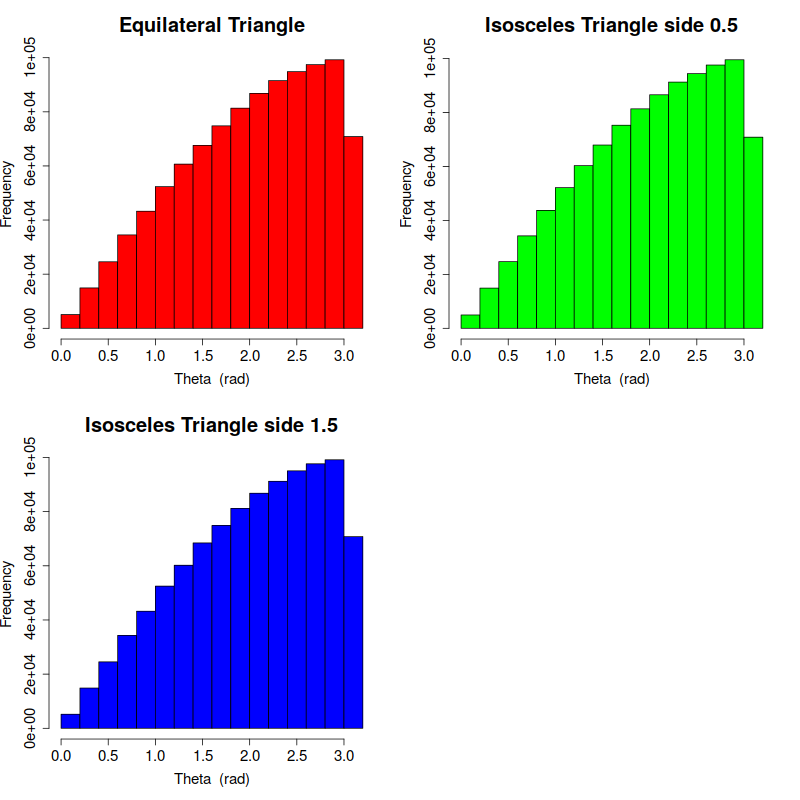
\includegraphics[width=400pt]{comp/hist.png}
  \label{fig:hist}
\end{figure}

There is no observable difference for a foil made of Isosceles Triangles of varying obtuseness.

\end{document}

